\subsubsection{\acl{la}}\label{subsec:local_aggregation}

% s. unten: Hyperparameter prob- woher? k, H ist getestet, zumindest das Verhältnis, aber lambda wird aus anderer Arbeit übernommen -> keine Hyperparameter Suche

\citet{local_aggr_2019} optimizes a low-dimensional feature space mapping by 
iteratively identifying close neighbours and updating the embedding function.
This soft clustering technique is called \ac{la}.

At each step during training of the embedding function $f_\theta: \mathcal{X} \rightarrow \mathcal{Z}$, 
two sets of neighbours are identified for each datapoint's embedding $z_i$ 
which are illustrated in \autoref{fig:la_bi_ci}.
The first set $C_i$ contains $z_i$'s close neighbours in the feature space, while
the second set $B_i$ contains $z_i$'s background neighbours.
$B_i$ is used as a means to judge distance and similarity, 
while $C_i$'s members should be embedded closer to $z_i$.
In other words, $C_i$ can be considered the set of positive samples while 
$B_i$ denotes the set of negative samples.
The level of \ac{la} $L(C_i,B_i | \theta, x_i)$ 
characterizes the relative level of closeness within $C_i$ compared to $B_i$.
$L(C_i,B_i | \theta, x_i)$ should be maximized.

The set $B_i$ consists of the $k$ nearest neighbours of $z_i$ in terms of cosine distance 
in the feature space.
$k$ is a hyperparameter and \citet{local_aggr_2019} set $k=4096$.
In order to construct $C_i$, 
first $H$ $k$-means clusterings are performed with sligthly different conditions.
Then, all of $z_i$'s clusters are united to form $C_i$.
$H$ and $k$ are hyperparameters.
\citet{local_aggr_2019} find that more clusterings, i.e. higher $H$, leads to isotropic clusters since outliers which arise from random processes are averaged out.
Moreover, if $H$ is too high compared to the number of clusters $k$, the performance decreases.
They state that $H=3, k=10000$ and $H=10, k=30000$ are better values than $H=10, k=10000$ 
in terms of ResNet-18 nearest neighbour validation performance.

Finally, the level of \ac{la} $L(C_i,B_i | \theta, x_i)$ is defined as the negative log-likelihood 
of the feature space representation $z_i$ of $x_i$ being in $C_i$ given $B_i$, 
i.e., being recognized as a close neighbour given being recognized as a background neighbour.
The loss to minimize is $\mathcal{L} = L(C_i,B_i | \theta, x_i) + \lambda \left\| \theta \right\|^2$.
\citet{local_aggr_2019} choose to rely on hyperparameter settings from another work rather than conducting a hyperparameter search.

\begin{figure}[!htb] % h = here, t = top, b = bottom, p = page of floats
    \centering
    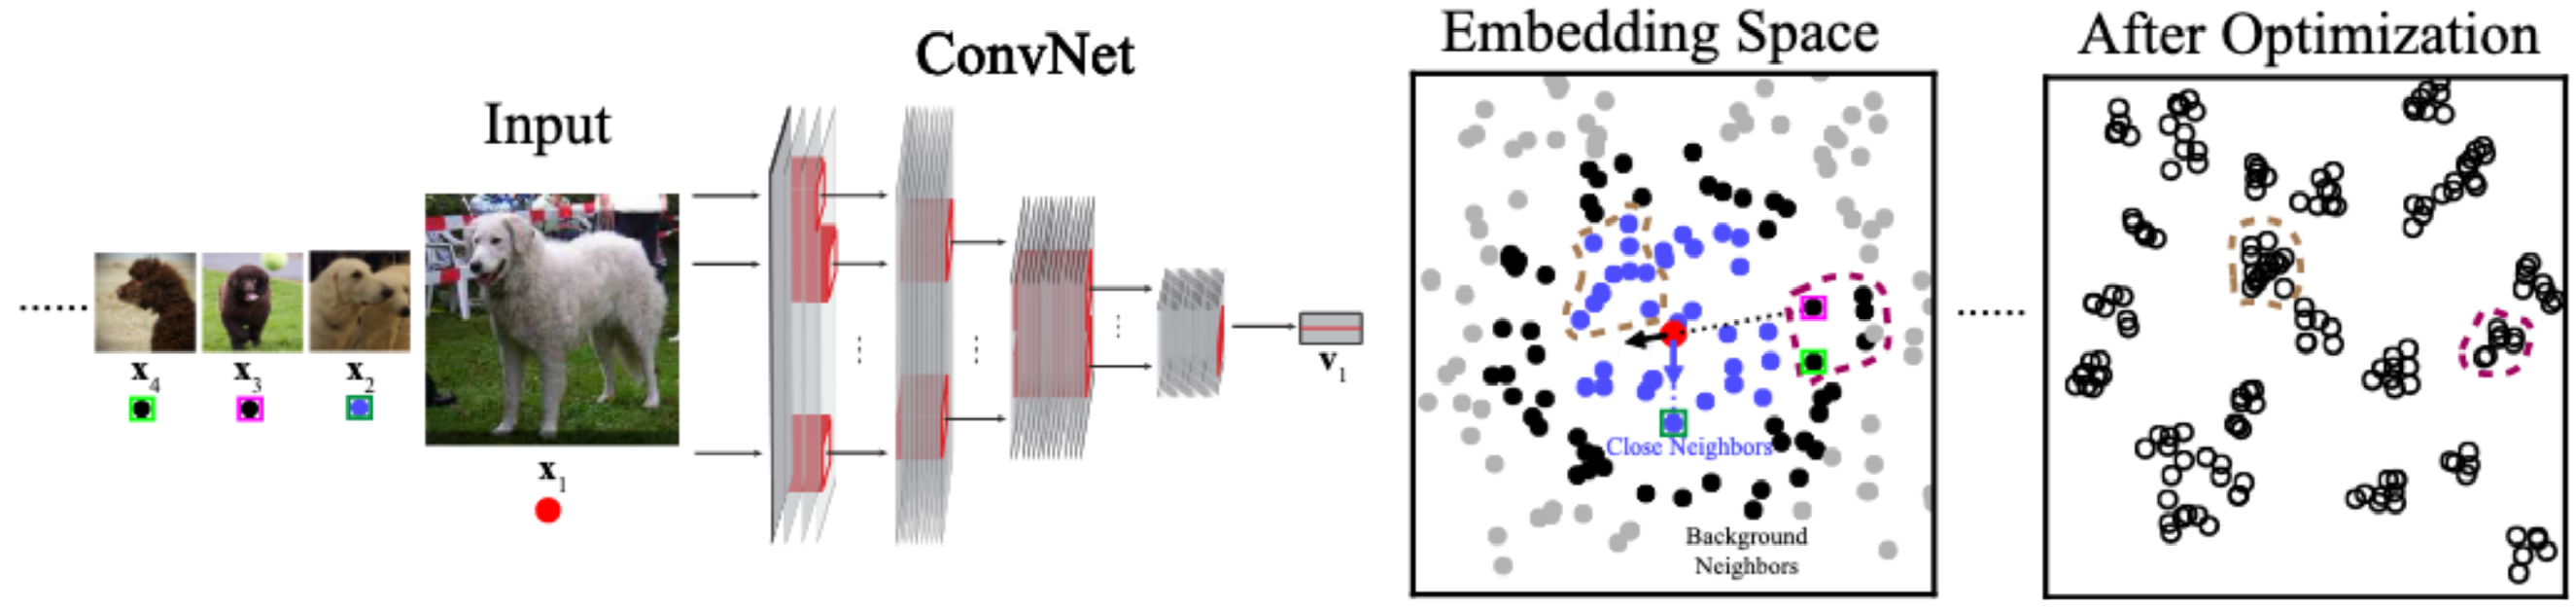
\includegraphics[width=360pt]{images/la_neighbourhoods.png}
    \caption{Illustration from \citet{local_aggr_2019}.
    A \ac{cnn} produces the feature space embedding $z_i = f_\theta(x_i)$.
    The embeddings are displayed as points in the feature space.
    The red point is the anchor $z_i$, 
    whereas blue points are close neighbours $C_i$ and
    black points are background neighbours $B_i$.
    The arrows denote influences between the neighbours.}
    \label{fig:la_bi_ci}
\end{figure}